\documentclass[11pt, a4paper, leqno]{article}
\usepackage{a4wide}
\usepackage[T1]{fontenc}
\usepackage[utf8]{inputenc}
\usepackage{float, afterpage, rotating, graphicx}
\usepackage{epstopdf}
\usepackage{longtable, booktabs, tabularx}
\usepackage{fancyvrb, moreverb, relsize}
\usepackage{eurosym, calc}
% \usepackage{chngcntr}
\usepackage{amsmath, amssymb, amsfonts, amsthm, bm}
\usepackage{caption}
\usepackage{mdwlist}
\usepackage{xfrac}
\usepackage{setspace}
\usepackage[dvipsnames]{xcolor}
\usepackage{subcaption}
\usepackage{minibox}
\usepackage{graphicx}
% \usepackage{pdf14} % Enable for Manuscriptcentral -- can't handle pdf 1.5
% \usepackage{endfloat} % Enable to move tables / figures to the end. Useful for some
% submissions.

\usepackage[
    natbib=true,
    bibencoding=inputenc,
    bibstyle=authoryear-ibid,
    citestyle=authoryear-comp,
    maxcitenames=3,
    maxbibnames=10,
    useprefix=false,
    sortcites=true,
    backend=biber
]{biblatex}
\AtBeginDocument{\toggletrue{blx@useprefix}}
\AtBeginBibliography{\togglefalse{blx@useprefix}}
\setlength{\bibitemsep}{1.5ex}
\addbibresource{/home/cheekoti_la/krishna/Generalised_Random_Forest_Methods/paper/refs.bib}


\usepackage[unicode=true]{hyperref}
\hypersetup{
    colorlinks=true,
    linkcolor=black,
    anchorcolor=black,
    citecolor=NavyBlue,
    filecolor=black,
    menucolor=black,
    runcolor=black,
    urlcolor=NavyBlue
}


\widowpenalty=10000
\clubpenalty=10000

\setlength{\parskip}{1ex}
\setlength{\parindent}{0ex}
\setstretch{1.5}


\begin{document}

\title{Generalised Random Forest Methods\thanks{Krishna Akolkar, University of Bonn. Email: \href{mailto:s6krakol@uni-bonn.de}{\nolinkurl{s6krakol [at] uni-bonn [dot] de}}.}}

\author{Krishna Akolkar}

\date{
    \\[1ex]
    \today
}

\maketitle


\begin{abstract}
    This project is an attempt to use Machine learning methods like Generalized Random Forest for asserting the hypothesis that
    ``fter the removal of ban on same-sex marriages in the USA in the span of 2004--2015, the same-sex married couples have increased''.
    The extention of this study is to understand whether such couples are encouraged to start a family.
    The motivation behind this
    study is a research paper by \textit{Susan Athey, Julie Tibshirani and Stefan Wager} on \href{https://arxiv.org/pdf/1610.01271}{Generalized Random Forest}
    I have used the methods discussed in the paper and tried to implement the methods on a different dataset.
    The aim of both the studies is to study the heterogeneous treatment effects on the dependent variable.
    I have used the EconML package by Microsoft to implement Causal Forest Double Machine Learning method on the dataset.
    With this approach, I calculate the treatment effects on the outcome and ultimately get the average treatment effect.

    A positive conditional average treatment effect stats that the policy intervention, or in our case, the removal of ban has a positive
    impact on the number of marriages in same-sex couples.
\end{abstract}

\clearpage


\section{Introduction}\label{sec:introduction}
 % (fold)

 Generalized Random Forest is a method for non-parametric statistical estimation based on random forest that can be used to fit any quantity
 of interest identified as the solution to a set of local moment equations.
 In this study, I will focus on the specific technique of causal forests, a causal machine learning method developed by economists, Susan Athey and Stefan Wager.
 Causal forests are similarly built as random forest, except that instead of minimizing prediction error which the random forest does, in causal forest, the data is split in order to
 maximize the difference across splits in the relationship between an outcome variable and a treatment variable.

Causal forest is a special case of generalized random forests.
When the treatment assignment W is binary and unconfounded, we have the conditional average treatment effect, $\tau(X) = E[Y(1) - Y(0) | X = x]$ where $Y(0)$ and $Y(1)$ are potential outcomes
corresponding to the two possible treatment states.
The main aim of causal forests is to understand the heterogeneous treatment effects across the sample.
A treatment effects can be understood a causal effect of a treatment or intervention on an outcome variable of interest.
 As individual treatment effects are unobservable, this practice focuses on estimating unbiased and consistent averages of the individual treatment effect.
 The most common parameter therefore is the average treatment effect, which is the mean of all individual treatment effects in the entire population of
interest.
However, sometimes treatment effects may vary widely between different subgroups in the population.
In some cases, it might therefore be more interesting to estimate these different, i.e.heterogeneous treatment effects.

 The dataset in this research study is extracted from \href{https://usa.ipums.org/usa/index.shtml}{IPUMS USA} which is a US Census microdata
 provider supported by University of Minnesota, USA. I extracted the data samples for the years 2010 to 2019 with various important variables.
 This dataset is a representative sample of the US Census.
 The authors of the research study mentioned previously have created an R package
 called \href{https://github.com/grf-labs/grf}{grf} which encompasses all the methods of non-paramatric estimation.
 For my study, I have used Microsoft's \href{https://github.com/py-why/EconML}{EconML} which uses python as the programming language.



 \section{Data and Variables} % (fold)
\label{sec:Data and Variables}

The years 2004 to 2015 have seen major changes in legislation regarding same-sex couples.
These changes mainly focus on legalizing and removing the ban on same-sex marriages and encouraging such marriages.
My major interest of study was to understand whether the same-sex couples, after such removing of bans, have really increased or not.
However, the US Census doesn't document live-in couples, it documents married couples.
So,I sought to wonder whether same-sex marriages have increased or not.
The dataset used in this study ranges from 2010 to 2019 which encompasses years having bans in some states and years after the removal of the same.

The 2nd hypothesis of this study is that ``Due to the removal of ban on same-sex marriages, number of such couples starting a family (own or
adopted) have increased''.
So, the outcome variable is whether the child in the family was born after 2015 or not.
A drawback or further refining
on this hypothesis is needed as I couldn't quantify the case of adopted children,i.e, at what age the child was adopted is not known.
Additionally, the treatment and instrument variables remain the same for this hypothesis.

$n = 50,179$

The key variables are, namely,
\begin{itemize}
    \item \textbf{features}($X_i$): include variables like SEX, RACE, EDUC(Education), EMPSTAT(Employment Status) and AGE.
    \item \textbf{features2}($X2_i$): include variables like SEX, RACE, EDUC(Education), EMPSTAT(Employment Status), AGE and
                                    NCHILD(no. of children in the family).
    \item \textbf{treatment}($T_i$): treatment variable is whether the couple is a same-sex couple. The treatment assignment is
     \[T_i=\begin{cases}
               1, & \text{if they are a same-sex couple}.\\
               0, & \text{otherwise}.
                   \end{cases}\]
    \item \textbf{instrument}($W_i$): instrument variable is such a variable which has some influence on the received treatment and thus on
                                    the outcome. The instrument variable here is INCTOT(Total Personal Income)
    \item \textbf{outcome}($Y_i$): outcome variable is whether the couple got married after 2015.
     \[Y_i=\begin{cases}
               1, & \text{if the couple got married after 2015}.\\
               0, & \text{otherwise}.
                   \end{cases}\]
    \item \textbf{outcome2}($Y2_i$): outcome variable is whether the child was born after 2015.
     \[Y_i=\begin{cases}
               1, & \text{if child birth after 2015}.\\
               0, & \text{otherwise}.
                   \end{cases}\]
\end{itemize}


 \section{Understanding the Model} % (fold)
\label{sec:Understanding the Model}

A causal forest is an average of many causal trees where the main difference comes due to subsampling
(\href{https://www.annualreviews.org/doi/abs/10.1146/annurev-economics-080217-053433}{Athey \& Imbens,2019})
To create a causal forest from
causal trees, it is necessary to estimate a weighting function and use the resulting weights to solve a local generalized method of moments (GMM)
model to estimate the conditional average treatment effect or CATE. To deal with overfitting, causal forests use an honesty condition, whereby a
tree is honest, if for each training sample $(i)$ it only uses the response $(Y)$ to estimate the within-leaf treatment effect or to decide where
to place the split, but not both.

To understand the causal model, I tried to visualize the model and its variables using the CausalModel package from the DoWhy library.
The model
can be seen in the Figure 1 (a and b).

\begin{figure}[!tbp]
  \begin{subfigure}[b]{0.5\textwidth}
    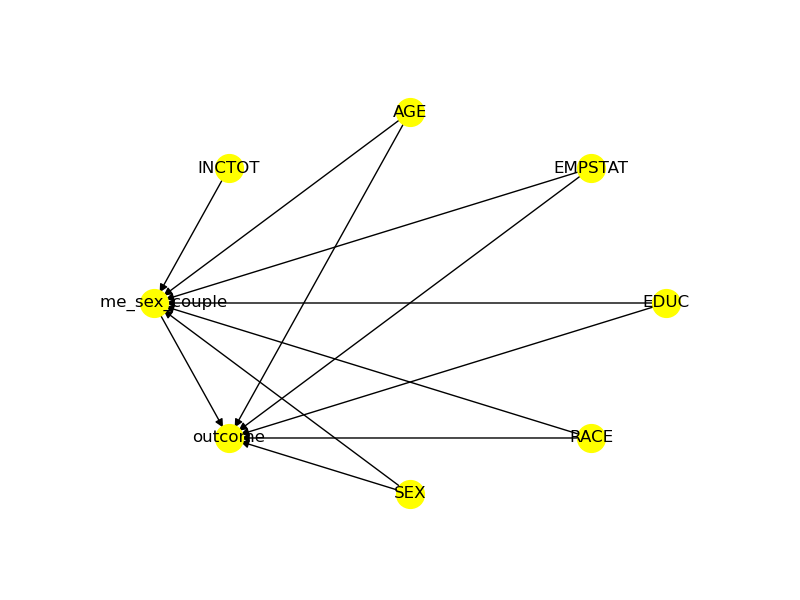
\includegraphics[width=\textwidth]{/home/cheekoti_la/krishna/Generalised_Random_Forest_Methods/bld/python/plots/causal_model}
    \caption{Causal Model for 1st hypothesis.}
    \label{fig:f1}
  \end{subfigure}
  \hfill
  \begin{subfigure}[b]{0.5\textwidth}
    \includegraphics[width=\textwidth]{/home/cheekoti_la/krishna/Generalised_Random_Forest_Methods/bld/python/plots/child_causal_model}
    \caption{Causal Model for 2nd hypothesis}
    \label{fig:f2}
  \end{subfigure}
  \caption{Visualization of variables and outcome}
\end{figure}

We observe \textit{i = 1,...,n} independent and identically distributed subjects, each of whom has features $X_i$, an outcome $Y_i$, a recieved
treatment $T_i$ and an instrument $W_i$, where $\tau(X)$ is the causal effects of treatment on the outcome.


 \section{Results} % (fold)
\label{sec:Results}

\begin{figure}[!tbp]
  \begin{subfigure}[c]{0.5\textwidth}
    \includegraphics[width=\textwidth]{/home/cheekoti_la/krishna/Generalised_Random_Forest_Methods/bld/python/plots/treatment_effects_plot}
    \caption{Treatment effect on same-sex couple}
    \label{fig:f3}
  \end{subfigure}
  \hfill
  \begin{subfigure}[c]{0.5\textwidth}
    \includegraphics[width=\textwidth]{/home/cheekoti_la/krishna/Generalised_Random_Forest_Methods/bld/python/plots/children_treatment_effects_plot}
    \caption{Treatment effect on child-birth}
    \label{fig:f4}
  \end{subfigure}
  \caption{Treatment effects and confidence intervals}
\end{figure}

After fitting the causal forest model on the data, the treatment effects are plotted in the above figure 2 (a and b).
While training the causal forest model, criterion is set to `het' which specifies heterogeneous treatment effects, which helps in observing the heterogeneous effects of the
treatment on the outcome.

Figure 2(a) explains the outcome of 1st hypothesis. At first the CATE looks negative and just a stable line, however, as the observation increases,
 the model is better fitted on the dataset and able to capture the treatment effects. When the observations are relatively larger, the CATE is
 relatively positive. From the plot, it can be stated that if more observations are taken and the sample-size is increased in terms of years, we could
 get a proper picture of the impact of the policy intervention as it takes time to undergo social changes in the society.

Figure 2(b) explains the outcome of 2nd hypothesis. In the case of starting a family, we could see a trend starting from negative and improving
gradually. These results have an impact due to its relation with the 1st hypothesis as the treatment variable is the same as the 1st hypothesis.
Here, we need to discount for the fact that we are taking children into consideration by birth and not able to quantify the children who are adopted
years after their birth. These results would be more accurate if we can have that number as well and more generalizations can be made accordingly.

It is visible in both the hypothesis that the treatment effects gradually turns positive and the average treatment effect is also positive. A
positive treatment effects depicts that the intervention or the treatment is positively affecting the sample.

\section{Conclusion} % (fold)
\label{sec:Conclusion}

Generalised random forest is a versatile method for adaptive, local estimation in a wide variety of statistical models. I have used this method
in context of heterogeneous treatment effects estimation using causal forest approach. Causal machine learning has the potential to have a
significant impact on the application of econometrics. It has the capacity to handle complex casual hypothesis and design model to treat such
hypothesis. As every individual is different mentally, physically and emotionally, it is very important to understand the treatment effects with
the inclusion of heterogeneity in it.

This project is an attempt to understand the impact of freedom given to ones' choices in terms of marriage laws and the encouragement given to
these couples to start a family. This project is in a primary stage of understanding the situation and building a model on it. The challenges
include the case of adoption and the ambiguity in terms of time and age of child adoption. If we can build more specific variables which reduces
this ambiguity than the results will be more resilient and interpretable.

% section introduction (end)



\setstretch{1}
\printbibliography
\setstretch{1.5}


% \appendix

% The chngctr package is needed for the following lines.
% \counterwithin{table}{section}
% \counterwithin{figure}{section}

\end{document}
